\section{Markov Decision Processes (MDPs)}
\begin{frame}{}
    \LARGE Reinforcement Learning: \textbf{Markov Decision Processes (MDPs)}
\end{frame}

\begin{frame}[allowframebreaks]{Mathematical Formulation of the RL Problem}
    \begin{itemize}
        \item \textbf{Markov property:} The current state completely characterizes the state of the world; that is, the future is independent of the past given the present.
        \item \textbf{Defined by:} $(\mathcal{S}, \mathcal{A}, R, P, \gamma)$
        \begin{itemize}
            \item $\mathcal{S}$: set of possible states
            \item $\mathcal{A}$: set of possible actions
            \item $R(s,a)$: reward distribution given a (state, action) pair
            \item $P(s' \mid s, a)$: transition probability, i.e., distribution over next state given a (state, action) pair
            \item $\gamma$: discount factor
        \end{itemize}
        \item Assumes the \textbf{Markov property}: the next state depends only on the current state and action.
    \end{itemize}
\framebreak
    \begin{figure}
        \centering
        \fetchconvertimage{https://optimization.cbe.cornell.edu/images/thumb/e/e0/Markov_Decision_Process_Example_2.png/499px-Markov_Decision_Process_Example_2.png}{images/intro/mdp.png}{width=\textwidth,height=0.9\textheight,keepaspectratio}
    \end{figure}
\framebreak
    \begin{itemize}
        \item At time step $t = 0$, the environment samples the initial state $s_0 \sim p(s_0)$.
        \item Then, for $t = 0$ until termination:
        \begin{itemize}
            \item The agent selects action $a_t$.
            \item The environment samples reward $r_t \sim R(\cdot|s_t, a_t)$.
            \item The environment samples the next state $s_{t+1} \sim P(\cdot|s_t, a_t)$.
            \item The agent receives reward $r_t$ and next state $s_{t+1}$.
        \end{itemize}
        \item A policy $\pi$ is a function from $\mathcal{S}$ to $\mathcal{A}$ that specifies which action to take in each state.
        \item \textbf{Objective:} Find a policy $\pi^\star$ that maximizes the cumulative discounted reward: $\sum_{t \geq 0} \gamma^t r_t$.
    \end{itemize}
\framebreak
    \begin{itemize}
        \item The agent and the environment interact in a time-sequenced loop:
        \begin{itemize}
            \item The agent observes the current state and reward, then selects an action.
            \item The environment responds by producing the next state and a scalar reward.
        \end{itemize}
        \item Each state satisfies the \textbf{Markov property}:
        \begin{itemize}
            \item The next state and reward depend only on the current state and action.
            \item The current state captures all relevant information from the history.
            \item The current state is a sufficient statistic for predicting the future (given the action).
        \end{itemize}
        \item The goal of the agent is to maximize the expected sum of all future rewards by controlling the policy function $\pi: \mathcal{S} \rightarrow \mathcal{A}$.
        \item This setup forms a dynamic, time-sequenced control system under uncertainty.
    \end{itemize}
\end{frame}

\begin{frame}[allowframebreaks]{A Simple MDP: Grid World}

    \begin{figure}
        \centering
        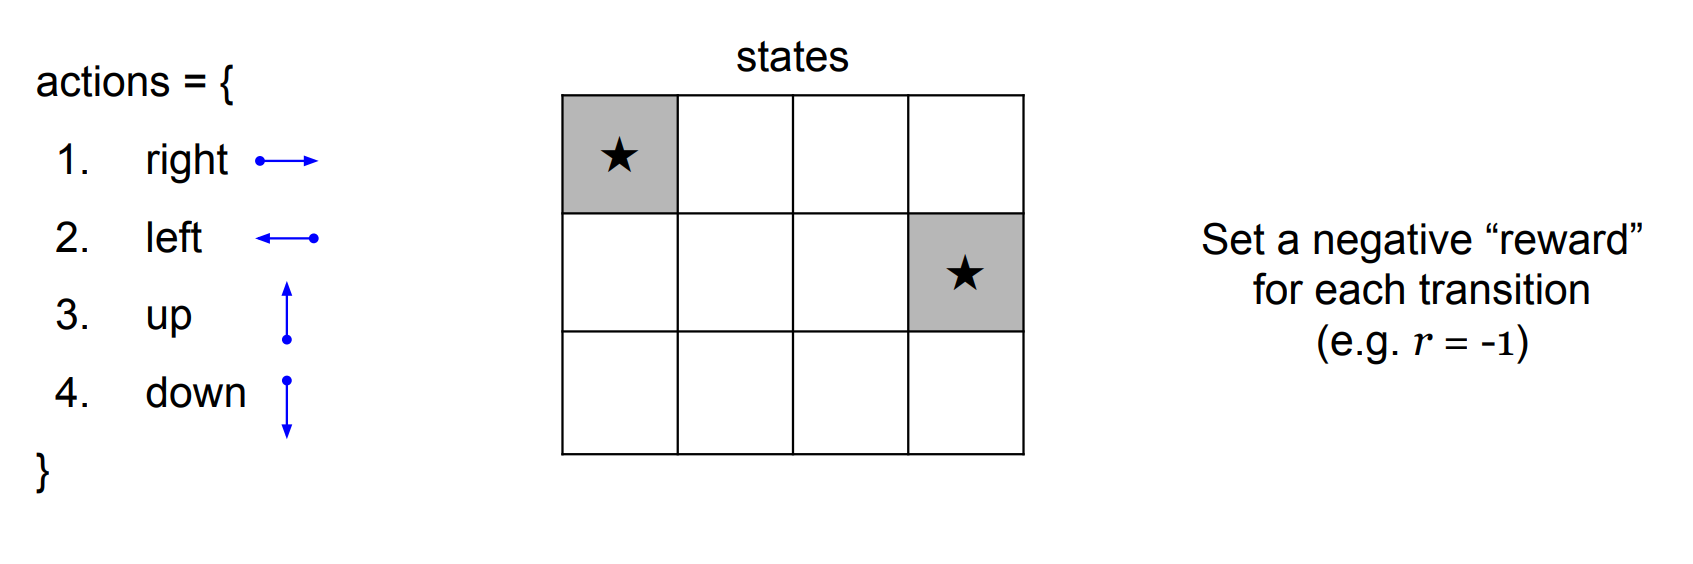
\includegraphics[width=0.9\textwidth,height=0.9\textheight,keepaspectratio]{images/intro/mdp_1.png}
    \end{figure}

    \centering
    \textbf{Objective}: Reach one of the terminal states (greyed out) in the least number of actions.

\framebreak

    \begin{figure}
        \centering
        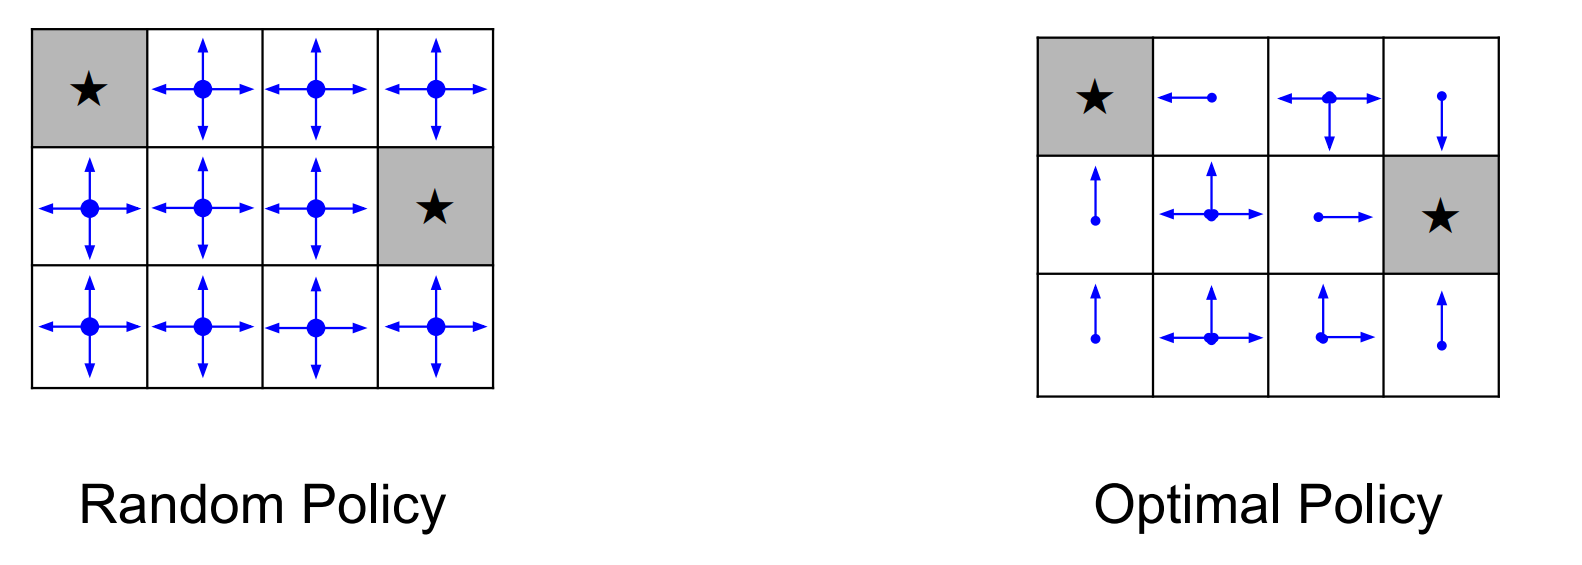
\includegraphics[width=0.9\textwidth,height=0.9\textheight,keepaspectratio]{images/intro/mdp_2.png}
    \end{figure}

\end{frame}

\begin{frame}{Real-World Problems that Fit the MDP Framework}
    \begin{itemize}
        \item Self-driving vehicles: choosing speed and steering to optimize safety and travel time
        \item Playing chess: receiving a reward only at the end of the game
        \item Complex logistical operations, such as managing movements in a warehouse
        \item Enabling a humanoid robot to walk or run on challenging terrains
        \item Managing an investment portfolio over time
        \item Controlling a power station efficiently
        \item Making optimal decisions during a football match
        \item Developing strategies to win an election (a high-complexity MDP)
    \end{itemize}
\end{frame}

\begin{frame}{Why Are These Problems Hard?}
    \begin{itemize}
        \item The state space can be large or complex (involving many variables).
        \item Sometimes, the action space is also large or complex.
        \item There is no direct feedback on “correct” actions (the only feedback is the reward).
        \item Time-sequenced complexity: actions influence future states and actions.
        \item Actions can have delayed consequences (delayed rewards).
        \item The agent often does not know the model of the environment.
        \item The “model” refers to the probabilities of state transitions and rewards.
        \item Thus, the agent has to learn the model and solve for the optimal policy.
        \item Agent actions need to trade off between “exploration” and “exploitation”.
    \end{itemize}
\end{frame}